%\documentclass[a4paper,10pt]{article}
\documentclass[10pt, conference, letterpaper]{algotel}
\usepackage[utf8]{inputenc}
\usepackage{xspace}
\usepackage{url}
\usepackage{graphicx,graphics} 
\usepackage{color}
\usepackage{amsmath}
\usepackage{amsfonts}
\usepackage{amssymb}
\usepackage{amsthm}
\usepackage{algorithm}
\usepackage{algorithmic}
\usepackage{longtable}
\usepackage{complexity}
\usepackage{tkz-graph}
\usepackage{float}
\usepackage{tabularx}
\usepackage{setspace}
\usepackage{icomma}
\usepackage{tkz-graph}
\usepackage{complexity}
\renewcommand{\algorithmicrequire}{\textbf{Input:}}
\renewcommand{\algorithmicensure}{\textbf{Output:}}
\usepackage[colorlinks=true,breaklinks=true,linkcolor=blue]{hyperref}


\newtheorem{proposition}{Proposition}
\newtheorem{theorem}{Theorem}

\setlength{\parskip}{1ex} % Espace entre les paragraphes

\newtheorem{fact}{Fact}
\newtheorem{lemma}[theorem]{Lemma}
\newtheorem{definition}{Definition}
\newtheorem{corollary}{Corollary}

% \renewcommand{\thefootnote}{\*}

\newcommand\pma{\textsc{pma}\xspace}
\newcommand{\todo}[1]{{\color{red} TODO: {#1}}}
\author{Maël Guiraud\addressmark{1,2}
  \and Yann Strozecki\addressmark{1}}

\address{\addressmark{1}David Laboratory, UVSQ, 45 Avenue des Etats Unis, Versailles France \\
  \addressmark{2}Nokia Bell Labs France, Route de Villejust, Nozay, France}


\title{Ordonnancement de messages périodiques sur un lien partagé}

\keywords{Periodic Scheduling, C-RAN, Greedy Algorithm, Latency} 
 

\begin{document}

\maketitle

%En français
%Ordonnancement de messages périodiques et de leurs réponses sur un lien partagé
\begin{abstract}
Le Cloud-RAN est une nouvelle architecture de réseau mobile dans laquelle les unités de calcul, traditionnellement installées au pieds des antennes, sont déportées dans des data-centers distants. Dans ces conditions, pour respecter des contraintes liées aux protocoles 4G et 5G, il faut minimiser la latence des messages périodiques envoyés par les antennes
à leurs unités de calcul. Nous essayons donc ici de trouver des plans périodiques de transmission des messages qui ne nécessitent pas de buffer et donc de latence supplémentaire.

Dans cet article nous étudions un lien partagé par toutes les antennes. Pour des messages arbitrairement grand, nous montrons qu'il existe toujours un plan de transmission des messages si la charge du réseau est inférieure à $40\%$.  Pour les messages de taille $1$, nous donnons un algorithme en temps polynomial qui trouve un plan de transmission pour des charges jusqu'à $61\%$. De plus, en analysant un algorithme aléatoire glouton, pour n'importe quelle charge, presque toutes les instances avec suffisamment de messages ont une solution, ce qui explique pourquoi les algorithmes gloutons présentés dans l'article marchent si bien en pratique.
\end{abstract}



%\begin{abstract}
%Cloud-RAN is a recent architecture for mobile networks where the processing units are located in distant data-centers while, until now, they were attached to antennas. The main challenge, to fulfill protocol time constraints, is to guarantee a low latency for the periodic messages sent from each antenna to its processing unit and back. The problem we address is to find a sending scheme of these periodic messages without contention nor buffering.

%We focus on a simple but common star shaped topology, where all contentions are on a single link shared by all antennas. For messages of arbitrary size, we show that there is always a solution as soon as the load of the network is less than $40\%$.
%For message of size $1$, we prove that it is always possible to schedule them, when the load is less than $61\%$  using a polynomial time algorithm. Moreover, using a simple random greedy algorithm, we show that almost all instances of a given load admit a solution, explaining why most greedy algorithms work so well in practice.  
%\end{abstract}

\section{Introduction and model}

Next generations of mobile network architectures evolve toward centralized radio network architectures called C-RAN for Cloud Radio Access Network, to reduce energy consumption costs~\cite{mobile2011c} and more generally the total cost of ownership. The main challenge for this type of architecture is to reach a latency compatible with transport protocols~\cite{ieeep802}. The specificity of the C-RAN context is not only the latency constraint, but also the periodicity of the data transfer in the frontaul network between RRHs and BBUs: messages need to be emitted and received each millisecond~\cite{bouguen2012lte}. Our aim is to operate a C-RAN on a low-cost shared switched network. Statistical multiplexing even with a large bandwidth does not satisfies the latency requirements of C-RAN~\cite{barth2018deterministic}. The current solution~\cite{tayq2017real} is to use dedicated circuits for the fronthaul but it does not scale in the case of a mobile network composed of about $10,000$ base stations. 

The question we address is the following: \emph{is it possible to schedule periodic messages on a shared link without using buffers}? Eliminating this source of latency leaves us with more time budget for latency due to the physical length of the routes in the network, and thus allows for wider deployment areas. Our proposed solution is to compute beforehand a \emph{periodic and deterministic} sending scheme, which completely avoids contention. 

We now formally describe our model and problem.
The time is discretized and the process we consider is periodic of fixed integer period $P$. In the C-RAN network we model, all messages are of the same nature, hence they are all of the same size denoted by $\tau$. This size corresponds to the time needed to send a message through some contention point of the network, here a link shared by all antennas. We denote by $n$ the number of messages, which are numbered from $0$ to $n-1$. A message $i$ is characterized by its delay $d_i$: if $i$ arrives at the link at time $t$, then it returns to the other end of the link on its way back at time $t + d_i$. 

Since the process we describe is periodic, we may consider any interval of $P$ units of time
to represent the state of our system. Describing the messages going through the two contention points during such an interval completely defines the periodic process. We call the representation of the interval of time in the first contention point the \emph{first period} and the \emph{second period} for the second contention point.

An \emph{offset} of a message is a choice of time at which it arrives
at the first contention point. Let us consider a message $i$
of offset $o_i$, it uses the interval of time $[i]_1 = \{ (o_i + t) \mod P \mid 0 \leq t < \tau \}$ in the first period and $[i]_2 = \{ (d_i + o_i + t) \mod P \mid 0 \leq t < \tau \}$ in the second period. We say that two messages $i$ and $j$ collide if either $[i]_1 \cap [j]_1 \neq \emptyset $ or $[i]_2 \cap [j]_2 \neq \emptyset $. If $t \in [i]_1$ (resp. $t \in [i]_2$) we say that message $i$ uses time $t$ in the first period (resp. in the second period).

We want to send all messages, so that they are no collision in the shared link.
In other word, we look for a way to send the messages without using buffering and 
hence limiting the latency to the physical length of the links. An \emph{assignment} is a
choice of an offset for each message such that \emph{no pair of message collide}, as shown in Fig.~\ref{fig:assignment}.  
We call Periodic Message Assignment or \pma the problem studied in this article,
which asks, given an instance of $n$ messages, a period $P$ and a size $\tau$, to find 
an assignment or to decide there is none.
\begin{figure}
\begin{center}
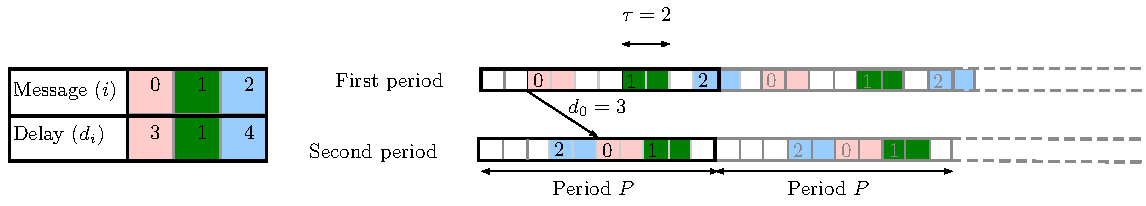
\includegraphics[scale=0.7]{instance}
\end{center}
\caption{An instance of \pma ($n=3$, $P= 10$, $\tau = 2$) and one assignment}
\label{fig:assignment}
\end{figure}
In previous articles of the authors, generalizations of \pma allowing buffers are studied on a single link~\cite{barth2018deterministic} or on a cycle~\cite{Guir1905:Deterministic}. Heuristics (using scheduling algorithms) and FPT algorithms are used to find a sending scheme with \emph{minimal latency}, while here we only look for sending scheme without any additional latency. More complex problems of computing schedules for time sensitive networks, such as sensor networks inside a car or a plane, have been practically solved~\cite{nayak2017incremental,steiner2018traffic}. 

The complexity of \pma is not yet known but slight variations are \NP-hard~\cite{barth2018deterministic}.  Hence, we conjecture that \pma is \NP-hard.
To overcome this supposed hardness, we study \pma when the load of the system is small enough. The \emph{load} is defined as the number of units of time used in a period by all messages divided by the period: $n\tau /P$. Our aim is to prove that, for small load, there is \emph{always} an assignment and that it can be found by a polynomial time algorithm.

All details, proofs, experiments lacking in this article can be found in~\cite{}.

\section{Greedy Algorithms for Large Messages} \label{sec:large}

In this section, we study the case of large messages. To prove that algorithms are able to build an assignment incrementally, we study $Fo(A)$ the maximum number of forbidden offsets when extending $A$ by some route.
Since $Fo(A)$ is always bounded by $(4 \tau -2)|S|$ where $S$ is the domain of $A$, any greedy algorithm succeeds when $(4 \tau -2)n \leq P$, that is when the load $n\tau /P$ is less than $1/4$. Two simple algorithms yields a better bound on $Fo(A)$.

The \emph{First Fit} algorithm deals with the route in the order they are given:  for each unscheduled route it tests all offsets from $0$ to $P-1$ until one do not create a collision with the current assignment. It turns out that First Fit always creates compact assignments (as defined in~\cite{barth2018deterministic}), that is a message is always next to another one in one of the two periods, which yields a better bound on $Fo(A)$.

A \emph{meta-offset} is an offset of value $i\tau$, with $i$ an integer from $0$ to $P / \tau$. We call Meta-Offset the greedy algorithm which works as First Fit, but consider only meta-offsets when scheduling new messages, see~\cite{barth2018deterministic}.

\begin{theorem}
First Fit and Meta-Offset always solves \pma positively on instances of load less than $1/3$.
\end{theorem}

 We try to combine the good properties of the two previous algorithms: the compacity of the assignments produced by First Fit and the use of meta-offsets to reduce collisions on the first period. The idea is to schedule several messages at once, using meta-offsets, to maximize the compacity of the obtained solution. 

 We consider the remainder modulo $\tau$ of the delays of each message. We write $d_i = d_{i}'\tau + r_i$ and assume from now on that messages are sorted by increasing $r_i$. A \emph{compact pair} is a pair of messages $(i,j)$ with $i < j$ such that we can put them next to each other in the second period using meta-offsets.
We have $r_i \leq r_j$ since $i < j$. We denote by $g$ the gap between the two messages in the first period, that we define by $d_{i}' = g + 1 + d_{j}' \mod m$. We require that $g \neq 0$ so that there are no collision in the first period if we schedule these two messages such that the difference of their offsets is the gap. 


We call \emph{Compact Pairs} the following greedy algorithm. From the $n$ routes in order
of increasing $r_i$, we build a sequence of at least $n/3$ compact pairs. They are then scheduled in the order they have been built using meta-offsets only. If at some point all compact pairs are scheduled or the current one cannot be scheduled, the remaining messages are scheduled as in Meta-Offset. The analysis of the algorithm relies on the evaluation of the number of forbidden meta-offsets. When scheduling a single message, a scheduled compact pair only forbids \emph{three} meta-offsets in the second period. If messages in a pair are scheduled independently, they forbid \emph{four} meta-offsets, which explains the improvement from Meta Offset.

\begin{theorem}
Compact Pairs always solves \pma positively on instances of load less than $3/8$.
\end{theorem}

Experimental results over random instances shows that all algorithms perform better than the worst case bounds given in the section. Compact Pair, which is the best theoretically also performs the best in our experiment, always finding assignments for load of $0.6$. 

 \section{Messages of Size One} \label{sec:small}

When $\tau = 1$, \emph{any greedy algorithm} finds a solution to \pma when the load is less than $1/2$ since $Fo(A) \leq (4\tau -2)|S| = 2|S|$ where $S$ is the number of scheduled messages. We now describes a method which always finds a solution for load of $1/2 + (\sqrt{5}/2 -1)$.
 
\begin{definition}
The potential of a message of delay $d$, for a partial assignment $A$
is the number of integers $i \in [P]$ such that $i$ is used in the first period and $i+d \mod P$ is used in the second period.
\end{definition}

The \emph{potential of a message} counts favorable configurations in terms of forbidden offsets.
When $i$ is used in the first period and $i+d \mod P$ is used in the second period,
then the same offset is forbidden \emph{twice} for a message of delay $d$. 
We define a global measure of quality of a partial assignment, 
that we try to maximize. This measure is \emph{the potential of an assignment}, denoted by $Pot(A)$, it is the sum of potentials for $A$ of all messages in the instance.

The \emph{potential of a position} $i$, for a partial assignment $A$, is the number of messages of delay $d$ such that $i+d \mod P$ is used by a route scheduled by $A$. 
Instead of decomposing the global potential as a sum over the messages, it can be understood
as a sum over positions. Hence, the sum of potentials of all positions used in the first period by messages scheduled by $A$ is equal to $Pot(A)$.  Moreover, the sum of potentials of all positions for a partial assignment with $k$ scheduled messages is $nk$.  

In the algorithm we propose, we guarantee to obtain $nk/2$ of potential by an exchange mechanism, that we call a swap. Let $A$ be some partial assignment of size $s$ and let $i$ be an unscheduled message of delay $d$. Assume that $i$ cannot be used to extend $A$. The swap operation is the following: select a free position $o$ in the first period, remove the message which uses the position $o+d$ in the second period from $A$ and extend $A$ by $i$ with offset $o$. We denote this operation by $Swap(i,o,A)$.

\begin{lemma}\label{lemma:swap}
Let $A$ be some partial assignment of size $k$ and let $i$ be an unscheduled message. If $i$ cannot be used to extend $A$, then either $Pot(A) \geq kn/2$ or there is an $o$ such that $Pot(Swap(i,o,A)) > Pot(A)$.
\end{lemma}

The \emph{Swap} algorithm is as follows: Schedule unscheduled messages while possible and then apply Swap operations while it increases the potential. When the potential is maximal, it tries to schedule a new message by moving one or two scheduled messages to new offsets. If it fails to find such messages the algorithm stops, otherwise it repeats the same steps. 

\begin{theorem}
The Swap algorithm solves positively \pma for instances with $\tau =1$ and load $1/2 + (\sqrt{5}/2 -1) \approx 0,618$.
\end{theorem}

Amazingly, in experiments Swap always finds an assignment when the load is less than $0.95$, but it is not always able to find assignments obtained by an exact resolution. 

We would like to understand better the behaviour of our algorithms
on instances drawn uniformly at random. To this aim, we analyze \textbf{Greedy Uniform}: for each message in order, choose one of the possible offsets uniformly at random and use it to extend the partial assignment. We compute the probability of success of Greedy Uniform over all random choices of the algorithm \emph{and all possible instances}. For a given assignment, we are only interested in its trace: the set of times which are used in the first and second period. Hence, if $n$ messages are scheduled in a period of size $m$, a trace of an assignment is a pair of subsets of $[m]$ of size $n$.

\begin{theorem}
The distribution of traces of assignments produced by Greedy Uniform when it succeeds, from instances drawn uniformly at random, is also uniform.
\end{theorem}

From the previous theorem, we can evaluate the probability that Greedy Uniform fails.

\begin{theorem}\label{theorem:uniform}
The probability over all instances with $n$ messages and period $m$ that Greedy Uniform solves $\pma$ positively is $\displaystyle{\prod_{i=m/2}^{n-1}(1 - \frac{\binom{n}{2i-m}}{\binom{m}{i}})}$.
\end{theorem}

Let $\lambda$, be the load, we can prove using Stirling formula that
$P(m,n) C \lambda m f(\lambda)^m$ with $f(\lambda) < 1$. Thus, the probability that Greedy Uniform fails goes to $0$ when $m$ grows. 

%\section{Lower bounds}

%Pour m=6, on peut toujours placer 5 éléments, que dire pour plus grand ?
%Remarque si tous les delais sont différents, on peut les placer, expliquer ça. 
%Example/family of examples for which some greedy alg fail -> facile pour le first fit
%Example/family of examples with a given load such that there are no feasible solution.
\bibliographystyle{alpha}
 \bibliography{Sources}

\end{document}
